%Our click model is designed for CTR prediction of display advertising. The observations of this application are Users' profile information, Ads' static attributes, and Users' behavior history. Different from the sponsored search, users come into display advertising system without clear target. Thus we wish to mining users' interest from the context information and estimate the CTR of each display accurately.
\section{Deep Interest Network}\label{sec:opa}

Different from sponsored search, users come into display advertising system without explicitly expressed intentions. 
Effective approaches are required to extract user interests from rich historical behaviors when building the CTR prediction model. 
Features that depict users and ads are the basic elements in the CTR modeling of advertisement system. 
Making use of these features reasonably and mining information from them are critical.

\subsection{Feature Representation}
Data in industrial CTR prediction tasks is mostly in a multi-group categorial form, for example, [weekday=Friday, gender=Female, \\ visited$\_$cate$\_$ids=$\{$Bag,Book$\}$, ad$\_$cate$\_$id=Book],
which is normally transformed into high-dimensional sparse binary features via encoding \cite{deep_crossing,widedeep,ftrl}. 
Mathematically, encoding vector of i-th feature group is formularized as $\textbf{t}_i \in R^{K_i}$. $K_i$ denotes the dimensionality of feature group $i$, which means feature group $i$ contains $K_i$ unique ids. 
$\textbf{t}_i[j]$ is the j-th element of $\textbf{t}_i$  and $\textbf{t}_i[j] \in \{0,1\}$. $\sum_{j=1}^{K_i} \textbf{t}_i[j]=k$. 
Vector $\textbf{t}_i$ with $k=1$ refers to one-hot encoding and $k>1$ refers to multi-hot encoding. 
Then one instance can be represent as $\bs{x} = [\bs{t}_1^T, \bs{t}_2^T,...\bs{t}_M^T]^T$ in a group-wise manner, where $M$ is number of feature groups, $\sum_{i=1}^{M}K_i = K$, $K$ is dimensionality of the entire feature space. 
In this way, the aforementioned instance with four groups of features are illustrated as: 
%\begin{equation}
\[
%  \underbrace{a + \overbrace{b+\cdots}^{{}=t}+z}_{\text{total}} ~~ a + {\overbrace{b+\cdots}^{126}+z
\underbrace{[0,0,0,0,1,0,0]}_{\text{weekday=Friday}} ~ \underbrace{[0,1]}_{\text{gender=Female}} ~ \underbrace{[0,..,1,...,1,...0]}_{\text{visited\_cate\_ids=\{Bag,Book\}}} 
~ \underbrace{[0,..,1,...,0]}_{\text{ad\_cate\_id=Book}}
\]
%\end{equation}

The whole feature set used in our system is described in Table \ref{table_feature_set}.
It is composed of four categories, among which user behavior features are typically multi-hot encoding vectors and contain rich information of user interests. 
Note that in our setting, there are no combination features. We capture the interaction of features with deep neural network. 

\begin{table}
\caption{Statistics of feature sets used in the display advertising system in Alibaba. Features are composed of sparse binary vectors in the group-wise manner.} % The dimensionality of fine-grained $goods\_ids$ feature scales up to $10^9$.}
\centering
\resizebox{0.47\textwidth}{!}{%
\label{table:fea-table}
\begin{tabular}{llccc}
\toprule
Category & Feature Group & Dimemsionality & Type & \#Nonzero Ids per Instance\\ \toprule
\multirow{3}{7em}{User Profile Features }
& gender & 2 &  one-hot & 1  \\ \cline{2-5}
& age\_level & $\sim 10$ &  one-hot & 1  \\ \cline{2-5}
& ... & ... & ... & ...  \\ \midrule

\multirow{4}{7em}{User Behavior Features}
& visited\_goods\_ids& $\sim 10^9$ &  multi-hot & $\sim 10^3$  \\ \cline{2-5}
& visited\_shop\_ids& $\sim 10^7$ &  multi-hot & $\sim 10^3$  \\ \cline{2-5}
& visited\_cate\_ids& $\sim 10^4$ &  multi-hot & $\sim 10^2$  \\\midrule

\multirow{4}{7em}{Ad Features }
& goods\_id & $\sim 10^7$ &  one-hot & 1  \\ \cline{2-5}
& shop\_id & $\sim 10^5$ &  one-hot & 1  \\ \cline{2-5}
& cate\_id & $\sim 10^4$ &  one-hot & 1   \\ \cline{2-5}
& ... & ... & ... & ...  \\ \midrule

\multirow{3}{7em}{Context Features }
& pid & $\sim 10$ &  one-hot & 1  \\ \cline{2-5}
& time & $\sim 10$ &  one-hot & 1  \\ \cline{2-5}
& ... & ... & ... & ...  \\ \bottomrule
\end{tabular}}
\label{table_feature_set}
\end{table}


\begin{figure*}[!t]
\centering
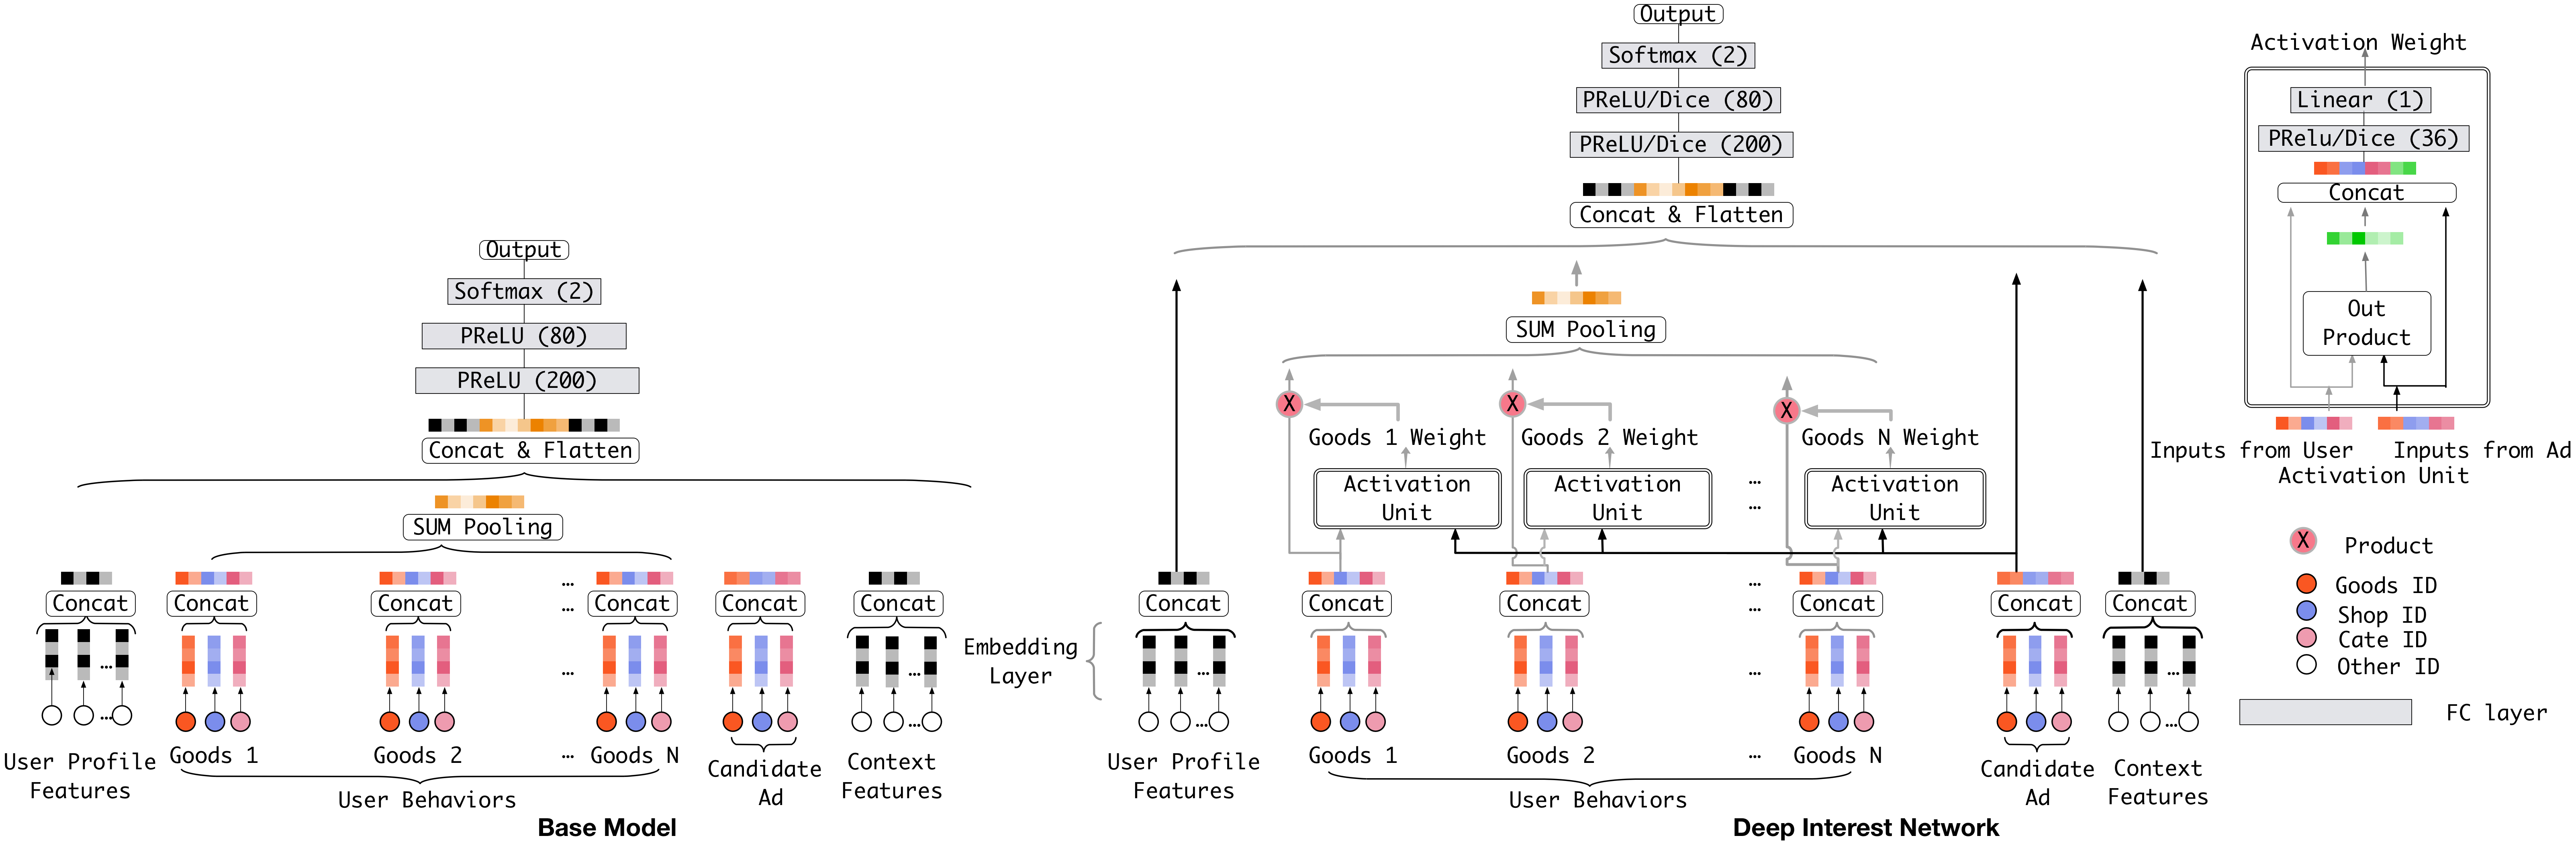
\includegraphics[height=7in, width=7in,keepaspectratio]{images/omni/DIN_new.png}
\caption{Network Architecture. The left part illustrates the network of base model (Embedding\&MLP). Embeddings of cate\_id, shop\_id and goods\_id belong to one goods are concatenated to represent one visited goods in user's behaviors. Right part is our proposed DIN model. It introduces a local activation unit, with which the representation of user interests varies adaptively given different candidate ads.}
\label{model_arch}
\end{figure*}


\subsection{Base Model(Embedding\&MLP)}
\label{sec:basemodel}
%Following the popular model structure introduced in \cite{deep_crossing,widedeep,youtube:recommend}, we design our base model as shown in the left of Fig.\ref{model_arch}.
Most of the popular model structures \cite{deep_crossing,widedeep,youtube:recommend} share a similar Embedding\&MLP paradigm, which we refer to as base model, as shown in the left of Fig.\ref{model_arch}. It consists of several parts:
%It follows the embedding\&MLP architecture. %, with all the parameters trained in the end-to-end manner.
\paragraph{\textbf{Embedding layer}} As the inputs are high dimensional binary vectors, embedding layer is used to transform them into low dimensional dense representations. 
%Let $\bs{t}_i\in \mathbb{R}^{K_i}$ represent the feature vector of i-th group in Table \ref{table_feature_set}. 
%Then one instance can be represent as $\bs{x} = [\bs{t}_1^T, \bs{t}_2^T,...\bs{t}_M^T]^T$ in a group-wise manner, where $M$ is number of feature groups, $\sum_{i=1}^{M}K_i = K$, $K$ is dimensionality of the entire feature space. 
For the i-th feature group of $\bs{t}_i$,  let $\mathrm{W}^i = [w_1^i,...,w_j^i, ..., w_{K_i}^i] \in\mathbb{R}^{D \times K_i}$ represent the i-th embedding dictionary, where $w_j^i \in R^D$ is an embedding vector with dimensionality of $D$.  
%Given instance of $\bs{x} = [\bs{t}_1^T, \bs{t}_2^T,...\bs{t}_M^T]^T$.
Embedding operation follows the table lookup mechanism, as illustrated in Fig.\ref{model_arch}. 
\begin{itemize}
\item If $\bs{t}_i$ is one-hot vector with j-th element $\bs{t}_i[j]=1$, the embedded representation of $\bs{t}_i$ is a single embedding vector $\bs{e}_i = w_j^i$. 
\item If $\bs{t}_i$ is multi-hot vector with $\bs{t}_i[j]=1 ~\text{for}~ j \in \{i_1, i_2, ..., i_k\} $, the embedded representation of $\bs{t}_i$ is a list of embedding vectors: $\{\bs{e}_{i_1}, \bs{e}_{i_2},...\bs{e}_{i_k}\} = \{w_{i_1}^i, w_{i_2}^i, ...w_{i_k}^i\}$.
\end{itemize}



\paragraph{\textbf{Pooling layer and Concat layer}} 
Notice that different users have different numbers of behaviors. Thus the number of non-zero values for multi-hot behavioral feature vector $\bs{t}_i$  varies across instances, causing the lengths of the corresponding list of embedding vectors to be variable.
As fully connected networks can only handle fixed-length inputs, it is a common practice \cite{widedeep,youtube:recommend} to transform the list of embedding vectors via a pooling layer to get a fixed-length vector: 
\begin{equation}
\label{eq:pooling}
\bs{e}_i = \text{pooling}(\bs{e}_{i_1}, \bs{e}_{i_2},...\bs{e}_{i_k}).	
\end{equation}
Two most commonly used pooling layers are sum pooling and average pooling, which apply element-wise sum/average operations to the list of embedding vectors. 

Both embedding and pooling layers operate in a group-wise manner, mapping the original sparse features into multiple fixed-length representation vectors.   
Then all the vectors are concatenated together to obtain the overall representation vector for the instance. 

\paragraph{\textbf{MLP}} Given the concatenated dense representation vector, fully connected layers are used to learn the combination of features automatically. 
Recently developed methods \cite{widedeep,DeepFM,PNN} focus on designing structures of MLP for better information extraction. \par
\paragraph{\textbf{Loss}}The objective function used in base model is the negative log-likelihood function defined as:
\begin{equation}
    L= - \frac{1}{N} \sum_{(\bs{x},y)\in\mathcal{S}} (y\log p(\bs{x}) + (1-y)\log(1-p(\bs{x}))),
\end{equation}
where $\mathcal{S}$ is the training set of size $N$, with $\bs{x}$ as the input of the network and $y\in \{0,1\}$ as the label, $p(\bs{x})$ is the output of the network after the softmax layer, representing the predicted probability of sample $\bs{x}$ being clicked.


\subsection{The structure of Deep Interest Network}

Among all those features of Table \ref{table_feature_set}, user behavior features are critically important and play key roles in modeling user interests in the scenario of e-commerce applications.   

Base model obtains a fixed-length representation vector of user interests by pooling all the embedding vectors over the user behavior feature group, as Eq.(\ref{eq:pooling}). This representation vector stays the same for a given user, in regardless of what candidate ads are.
In this way, the user representation vector with a limited dimension will be a bottleneck to express user's diverse interests.
To make it capable enough, an easy method is to expand the dimension of embedding vector, which unfortunately will increase the size of learning parameters heavily.
It will lead to overfitting under limited training data and add the burden of computation and storage, which may not be tolerated for an industrial online system. 

%As discussed above, when visiting e-commerce sites, users are often interested in many kinds of goods. 
%In other words, user interests are diverse.  
%However, it is known that users are often with diverse interests when visiting e-commerce sites. 
%Base model obtains the user interest vector by average pooling over the embedding of all behaviors. Thus base model obtains a same interest vector of users given different candidate ads for one user.
% In the base model, sums the embedding of all user behavior ids to obtain the user interest vector. The model obtains the same user % interest vector when predicts different candidate ad for one user.
%In order to embed diverse user interests in this vector, one easy method is expanding the dimension to make it capable enough to contain information of different interests. 
%Unfortunately, high dimension of embedding vectors will increase the size of learning parameters heavily.
%It will lead to overfitting under limited training data and add the burden of computation and storage, which may not be tolerated for an industrial online system.

Is there an elegant way to represent user's diverse interests in one vector under limited dimension?
The local activation characteristic of user interests gives us inspiration to design a novel model named deep interest network(DIN).
Imagine when the young mother mentioned above in section \ref{sec:bg} visits the e-commerce site, she finds the displayed new handbag cute and clicks it.
Let's dissect the driving force of click action. 
The displayed ad hits the related interests of this young mother by soft-searching her historical behaviors and finding that she had browsed similar goods of tote bag and leather handbag recently.  
In other words, behaviors related to displayed ad greatly contribute to the click action.  
DIN simulates this process by paying attention to the representation of locally activated interests w.r.t. given ad.
Instead of expressing all user's diverse interests with the same vector, DIN adaptively calculate the representation vector of user interests by taking into consideration the relevance of historical behaviors w.r.t. candidate ad.
This representation vector varies over different ads.         

The right part of Fig.\ref{model_arch} illustrates the architecture of DIN. 
Compared with base model, DIN introduces a novel designed local activation unit and maintains the other structures the same.  Specifically, activation units are applied on the user behavior features, which performs as a weighted sum pooling to adaptively calculate user representation $\bs{v}_U$ given a candidate ad $A$, as shown in Eq.(\ref{eq:attention})


%By simulating this process, we   
%Instead of focusing on a global representation vector, we actually only need to pay attention to the representation of locally related interests given a candidate ad.  
%In this way, representation vector of user interest is calculated adaptively given $\prec$user, ad$\succ$ pair. 
%That is, it varies over different candidate ads.  
%Then user vector only needs to represent related interest when faced different candidate ad, which is within the ability of a vector with appropriate dimension. \par
%For different candidate ads, we want our model to find related part of interests automatically. \par
%This candidate specific interest vector can be realized by attention mechanism\cite{bengio:attention}, which derive from neural machine translation.
%Under this consideration, we design a novel model named deep interest network(DIN), to better capture the characteristic of user behavior data and help improving the expressive ability of model under limited embedding dimension. 
%It is illustrated in the right of Fig.\ref{model_arch}.
%Compared with base model, DIN introduces a new designed activation unit and maintains the other net structures the same.  

%Specifically, activation unit is applied on the user behavior feature groups, which performs as a weighted average pooling to adaptively calculate user representation $\bs{v}_U$ given a candidate ad $A$, as shown in Eq.(\ref{eq:attention})
{
%\setlength\abovedisplayskip{1pt}
%\setlength\belowdisplayskip{1pt}
\begin{small}
\begin{eqnarray}
\begin{split}
\label{eq:attention}
\bs{v}_U(A) = f(\bs{v}_A,\bs{e}_1,\bs{e}_2,..,\bs{e}_H) & = \sum_{j=1}^H a(\bs{e}_j,\bs{v}_A) \bs{e}_j = \sum_{j=1}^H \bs{w}_j \bs{e}_j,
\end{split}
\end{eqnarray}
\end{small}
}
where $\{\bs{e}_1, \bs{e}_2, ..., \bs{e}_H\}$ is the list of embedding vectors of behaviors of user $U$ with length of $H$, $\bs{v}_A$ is the embedding vector of ad $A$. In this way, $\bs{v}_U(A)$ varies over different ads. $a(\cdot)$ is a feed-forward network with output as the activation weight, as illustrated in Fig.\ref{model_arch}. Apart from the two input embedding vectors, $a(\cdot)$ adds the out product of them to feed into the subsequent network, which is an explicit knowledge to help relevance   modeling.   

Local activation unit of Eq.(\ref{eq:attention}) shares similar ideas with attention methods which are developed in NMT task\cite{bengio:attention}.
However different from traditional attention method, the constraint of $\sum_i w_i = 1$ is relaxed in Eq.(\ref{eq:attention}), aiming to reserve the intensity of user interests. 
That is, normalization with softmax on the output of $a(\cdot)$ is abandoned.
Instead, value of $\sum_i w_i$ is treated as an approximation of the intensity of activated user interests to some degree.   
For example, if one user's historical behaviors contain 90\% clothes and 10\% electronics. 
Given two candidate ads of T-shirt and phone, T-shirt activates most of the historical behaviors belonging to clothes and may get larger value of $\bs{v}_U$ (higher intensity of interest) than phone. 
Traditional attention methods lose the resolution on the numerical scale of $\bs{v}_U$ by normalizing of the output of $a(\cdot)$. 
%Taking the original output of $a(\cdot)$  as activation score can be a simple way to maintain the intensity of interest, which helps making use of user historical behavior data more sufficiently.


%Assume user U is interested in clothes and electronics, with the intensity to be 90\% and 10\% relatively. 
%This causes the historical behaviors of clothes occur more \textbf{frequently} than electronics for $U$.     
%Assume two candidate ads T-shirt and iphone are selected as candidates for $U$.
%Value of representation vector $\bs{v}_U$ given T-shirt will be larger than given iphone.
%Indeed, taking the original output of $a(\cdot)$  as activation weight can be a simple way to maintain the intensity of interest, which helps us making use of user historical behavior more sufficiently.

We have tried LSTM to model user historical behavior data in the sequential manner.
But it shows no improvement. 
%But it makes little difference. 
Different from text which is under the constraint of grammar in NLP task, the sequence of user historical behaviors may contain multiple concurrent interests.
Rapid jumping and sudden ending over these interests causes the sequence data of user behaviors to seem to be noisy.
A possible direction is to design special structures to model such data in a sequence way.
We leave it for future research.  


%Meanwhile, user behavior is not only affected by his diverse interests but also depends on the results our system display. 
%In our attempt, directly modeling user behavior sequence with RNNs shows little improvement.  
%This makes it difficult for directly deploying the RNNs to model user behavior sequence in e-commerce scenario.

%It's notable that the value of $\bs{v}_U$ given candidate ad that relates to \textbf{frequent} historical behavior is larger than others. 
%For example, if one user's historical behavior contains 80\% clothes and 20\% electronics. For candidate ads: T-shirt and phone, more historical behaviors get high attention score for T-shirt, which leads to the value of vector $\bs{v}_U$ computed for the user is larger for T-shirt than for phone. It means the value of vector can reflect the user's interest intensity. But traditional attention methods that use normalization with softmax on the output of $a$ to scale the value of $\bs{v}_U$ into the same range is not suitable in our scenario, which may lose the information of interest intensity. Instead, the original output of $a$ can maintain the intensity of interest, which helps us making use of user historical behavior more sufficiently.

%It seems to be natural to use RNNs for modeling user interest by taking the sequence of user behaviors as inputs. 
%However, we implement it and find no difference. 
%A possible explanation is that different from text that is under the constraint of grammar, the sequence of user historical behaviors contains concurrent multiple varying interests and may rapidly jump over these interests, which make the sequence data to be disordered and noisy. 
%We leave this for future research. 
%Meanwhile, user's behavior is not only affected by his diverse interests but also another factors such as the results our system display. Thus the information about sequence in e-commerce scenario is much weaker than that in text.
 

%The use of attention makes users' diverse interest be captured. Further, these diversity interest can be local activated when predict one specific candidate ad.
%In all, DIN designs the activation unit to follow local activation structure and weighted sum pooling to follow diversity structure.
%To the best of our knowledge, DIN is the first model which follows both of the two structures of user behavior data in CTR prediction tasks at the same time.
%\subsection{Mini-batch Aware Regularization Technique}

\section{Training Techniques}
In the advertising system in Alibaba, numbers of goods and users scale up to hundreds of millions.  
%There are billion kinds of goods in Alibaba, and our advertising system needs to serve more than hundred million users one day.
Practically, training industrial deep networks with large scale sparse input features is of great challenge.
In this section, we introduce two important techniques which are proven to be helpful in practice. 

\subsection{Mini-batch Aware Regularization}

%In order to capture more specific interests of users, we typically introduce billions of fine-grained ids to describe the users' behaviors. These sparse and high dimensional features may lead to severe overfitting problem.
%{\EDIT why these feature would cause overfitting?(1 more parameter ; 2 less times)}
%to capture user interest detailly. \par
%Not surprisingly, overfitting problem is encountered while training our model with large scale parameters and sparse inputs.
%In experiment, with addition of fine-grained user visited $good\_ids$ feature, model performance falls rapidly after the first epoch.\par
%It is known that internet-scale user behavior data follows the long-tail law, that is, lots of feature ids occur a few times in the training samples, while little of them occur many times.
%This inevitably introduces noise into the training process and intensifies overfitting.
%An easy way to reduce overfitting is to filter out those low-frequency feature ids, which can be viewed as manual regularization.
%However, such frequency based filter is quite rough in terms of information loss and threshold setting.
%Many methods have been proposed to reduce overfitting, such as $\ell_2$ and $\ell_1$ regularization \cite{lasso}, and Dropout \cite{dropout}. 
%However, merely of them are suitable for training network with sparse inputs and billions of parameters.

%Practically overfitting problem is encountered while training industrial networks with large scale sparse input features.
Overfitting is a critical challenge for training industrial networks. 
For example, with addition of fine-grained features, such as features of $\textsl{goods\_ids}$ with dimensionality of 0.6 billion (including $visited\_goods\_ids$ of user and $goods\_id$ of ad as described in Table \ref{table_feature_set}), model performance falls rapidly after the first epoch during training without regularization, as the dark green line shown in Fig.\ref{fig:adaptive_reg} in later section \ref{sec:reg}.   
It is not practical to directly apply traditional regularization methods, such as $\ell_2$ and $\ell_1$ regularization, on training networks with sparse inputs and hundreds of millions of parameters.
Take $\ell_2$ regularization as an example.
Only parameters of non-zero sparse features appearing in each mini-batch needs to be updated in the scenario of SGD based optimization methods without regularization. 
However, when adding $\ell_2$ regularization it needs to calculate L2-norm over the whole parameters for each mini-batch, which leads to extremely heavy computations and is unacceptable with parameters scaling up to hundreds of millions.        
%Original $\ell_2$ regularization needs to calculated L2-norm over the whole parameters on each mini-batch, which leads to extremely heavy computations and is unacceptable in our situation. 

\begin{figure}[!ht]
%\setlength{\belowcaptionskip}{-0.5cm}
\centering
%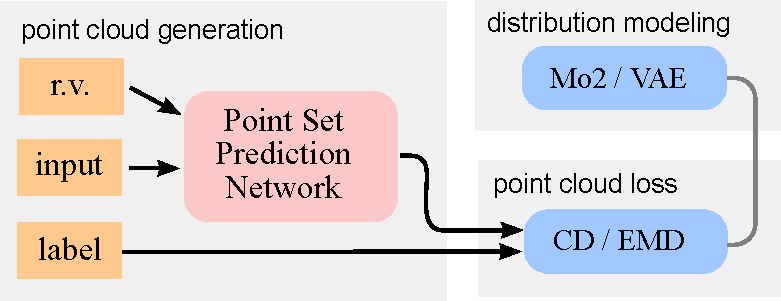
\includegraphics[height=4.5in, width=5in,keepaspectratio]{images/omni/system}
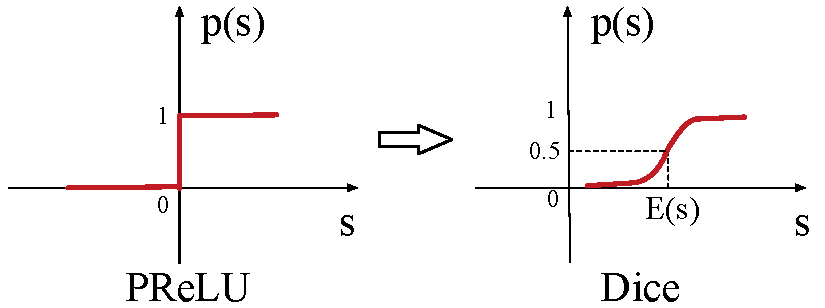
\includegraphics[height=1.8in, width=2.2in,keepaspectratio]{images/omni/dice_activation}
\caption{Control function of PReLU and Dice.}
\label{figure_dice}
\vspace{-0.4cm}
\end{figure} 


In this paper, we introduce an efficient mini-batch aware regularizer, which only calculates the L2-norm over the parameters of sparse features appearing in each mini-batch and makes the computation possible.     
In fact, it is the embedding dictionary that contributes most of the parameters for CTR networks and arises the difficulty of heavy computation. 
Let $\bs{\mathrm{W}}\in\mathbb{R}^{D\times K}$ denote parameters of the whole embedding dictionary, with $D$ as the dimensionality of the embedding vector and $K$ as the dimensionality of feature space. 
Expand the $\ell_2$ regularization on $\bs{\mathrm{W}}$ over samples 
%\begin{equation}
%\label{eq:batch}
%\sum_{i=1}^{n_{dj}} \frac{I_{id}}{n_{dj}}w_d^2
%\end{equation}
\begin{footnotesize}
\begin{eqnarray}
\begin{split}
\label{eq:batch}
L_2(\bs{\mathrm{W}}) &= \|\bs{\mathrm{W}}\|_2^2 = \sum_{j=1}^{K}\|\bs{w}_j\|_2^2 = \sum_{(\bs{x},y)\in\mathcal{S}}\sum_{j=1}^{K} \frac{I(\bs{x}_j\neq0)}{n_{j}}\|\bs{w}_j\|_2^2,
\end{split}
\end{eqnarray}
\end{footnotesize}
where $\bs{w}_j\in\mathbb{R}^{D}$ is the $j$-th embedding vector,
%which corresponding to the number of feature IDs in our applications.
$I(\bs{x}_j\neq0)$ denotes if the instance $\bs{x}$ has the feature id $j$, and $n_j$ denotes the number of occurrence for feature id $j$ in all samples. %Here we use $I(\cdot)$ as the indicator function.
%When applying the gradient descent optimization on mini-batches, the regularization is transformed into
Eq.(\ref{eq:batch}) can be transformed into Eq.(\ref{eq:minibatch}) in the mini-batch aware manner 
\begin{small}
\begin{equation}
\label{eq:minibatch}
L_2(\bs{\mathrm{W}}) = \sum_{j=1}^{K}\sum_{m=1}^{B}\sum_{(\bs{x},y)\in\mathcal{B}_m}\frac{I(\bs{x}_j\neq 0)}{n_{j}}\|\bs{w}_j\|_2^2,
\end{equation}
\end{small}
where $B$ denotes the number of mini-batches, $\mathcal{B}_m$ denotes the $m$-th mini-batch.
%To simplify the computation, 
Let $\alpha_{mj} = \max_{(\bs{x},y)\in\mathcal{B}_m} I(\bs{x}_j\neq0)$
%{\small
%\begin{equation}
%\alpha_{mj} = \max_{(\bs{x},y)\in\mathcal{B}_m} I(\bs{x}_j\neq0),
%\end{equation}}
denote if there is at least one instance having the feature id $j$ in mini-batch $\mathcal{B}_m$.
Then Eq.(\ref{eq:minibatch}) can be approximated by
\begin{small}
\begin{equation}
\label{eq:approx}
L_2(\bs{\mathrm{W}})\approx\sum_{j=1}^{K} \sum_{m=1}^{B}  \frac{\alpha_{mj}}{n_j}\|\bs{w}_j\|_2^2.
\end{equation}
\end{small}
In this way, we derive an approximated mini-batch aware version of $\ell_2$ regularization.
For the $m$-th mini-batch, the gradient w.r.t. the embedding weights of feature $j$ is
%\begin{equation}	
%\scalebox{0.9}{
%\parbox{0.37\textwidth}{
%\begin{eqnarray}
%\begin{split}
%\bs{w}_j \leftarrow \bs{w}_j- \eta
%    \left[
%       \frac{1}{|\mathcal{B}_m|} \sum_{(\bs{x},y) \in \mathcal{B}_m} { \frac{\partial L(p(\bs{x}), y)}{\partial \bs{w}_j}
%       +\lambda \frac{\alpha_{mj}}{n_j}\bs{w}_j}
%    \right].
%\end{split}
%\end{eqnarray}
%}
%}
%\end{equation}
\begin{small}
\begin{equation}
\bs{w}_j \leftarrow \bs{w}_j- \eta
    \left[
       \frac{1}{|\mathcal{B}_m|} \sum_{(\bs{x},y) \in \mathcal{B}_m} { \frac{\partial L(p(\bs{x}), y)}{\partial \bs{w}_j}
       +\lambda \frac{\alpha_{mj}}{n_j}\bs{w}_j}
    \right],
\end{equation}
\end{small}
in which only parameters of features appearing in $m$-th mini-batch participate in the computation of regularization. 

%Different from the regularization in~\cite{difacto}, our approach imposes more penalty on long-tail features(which is hard to learn) of lower frequency than frequent $goods\_id$(which may reflect user interests confidently). 
%Experiments show that our approach outperforms other regularization methods, like dropout.




% let $w_j$ denotes the parameter in embedding layer,
%In common, the gradient of loss  $L(x; W)$ combined with $L_2(W)$ to the embedding layer's parameter $W_{jk}$(the embedding matrix for the kth id of feature $X_j$)is
%\begin{equation}
%\label{ada-reg}
%W_{jk} \leftarrow W_{jk} - \eta
%    \left[
%       \frac{1}{b} \sum_{(x_i,y_i) \in B} { \frac{\partial L(f(x_i), y_i)}{\partial W_{jk}} +\lambda W_{jk}}
%    \right]
%\end{equation}
%Where $B$ stands for mini-batch samples with size of $b$.  $\lambda$ is regularization parameter.

%Many methods have been proposed to reduce overfitting, such as $L_2$ and $L_1$ regularization \cite{lasso}, and Dropout \cite{dropout}.
%However, with sparse and high dimensional data,  CTR prediction task faces greater challenge.
%It is known that internet-scale user behavior data follows the long-tail law, that is, lots of feature ids occur a few times in the training samples, while little of them occur many times.
%This inevitably introduces noise into the training process and intensifies overfitting.
%
%%According to our experience,
%An easy way to reduce overfitting is to filter out those low-frequency feature ids, which can be viewed as manual regularization.
%However, such frequency based filter is quite rough in terms of information loss and threshold setting.
%Here we introduce an adaptive regularization method, in which we impose different regularization intensity on feature ids according to their occurrence frequency.
%On realizing this method, we apply frequency related L2-norm regularization to good ids that actually occur in current mini-batch.
%The last term brings to some problem, on the one hand, it has effect on $W_{jk}$ even if $x_{ij}$ is 0. On the one hand, it improves the consumption of computation; On the other hand, it will lead error director for the update of $w_{e_j}$.\par
%
%In order to avoid extra updating, we try to introduce one control unit to the update when one batch using one specific id.
%Denote that,
%\begin{equation}
%I_i = \left\{ \begin{array}{ll}
%1, & \exists  (x_j,y_j) \in B, s.t. \left[ x_j \right]_i \neq 0\\
%0, & \textrm{other wises}
%\end{array} \right.
%\end{equation}
%
%\begin{equation}
%\label{ada-reg}
%W_{jk} \leftarrow W_{jk} - \eta
%    \left[
%       \frac{1}{b} \sum_{(x_i,y_i) \in B} { \frac{\partial L(f(x_i), y_i)}{\partial W_{jk}} +\lambda W_{jk}I_i}
%    \right]
%\end{equation}
% While there is another problem, the update times for different frequent feature is different, which means the regularization on low frequent feature is weak, which violates the goal.\par
% Aiming to solve this problem, we design an adaptive regularization method, which applies different regularization intensity on feature ids according to their occurrence frequency.
%Let's analyze the gradient updating from the aspect of instance.
%Aiming to solving this problems, we design an adaptive regularization method, which imposes different regularization intensity on feature ids according to their occurrence frequency.\par
%Denote that,
%\begin{equation}
%I_i = \left\{ \begin{array}{ll}
%1, & \exists  (x_j,y_j) \in B, s.t. \left[ x_j \right]_i \neq 0\\
%0, & \textrm{other wises}
%\end{array} \right.
%\end{equation}

%\begin{equation}
%\label{ada-reg}
%W_{jk} \leftarrow W_{jk} - \eta
%    \left[
%       \frac{1}{b} \sum_{(x_i,y_i) \in B} { \frac{\partial L(f(x_i), y_i)}{\partial W_{jk}} +\lambda \frac{1}{n_i}W_{jk}I_i}
%    \right]
%\end{equation}
%where $n_i$ is frequency of feature $i$.\par


%The idea behind Eq.(\ref{ada-reg}) is to penalize low-frequency features and relax high-frequency features to control the gradient update variance.
%When b is set to 1, the update is equivalent to dividing regularization term of full batch update onto each sample. When mini batch size is large than 1, we still use $\lambda \frac{1}{n_i}$ as regular coefficient to avoid counting good id's frequency in current mini batch.

%% PLAN A
%A similar practice of adaptive regularization can be found in \cite{difacto} which sets regular coefficient to be proportional to feature frequency where they
%, as shown below:
%\begin{equation}
%\label{limu}
%w_i \leftarrow w_i - \eta
%    \left[
%       \frac{1}{b} \sum_{(x_j,y_j) \in B} { \frac{\partial L(f(x_j), y_j)}{\partial w_i} +\lambda n_iw_iI_i}
%    \right]
%\end{equation}
%However, in our dataset, training with regularization of Eq.(\ref{limu}) shows no obvious alleviation of overfitting. On the contrary, it slows down the convergence of training process. Eq.(\ref{limu}) applies greater penalty on high-frequency good ids than long-tail goods, while the former contributes more on both the metric and online income in our special e-commerce system. Besides, we also evaluate dropout technique and find slight improvement on overfitting.
%However, when we train DNN model on our display advertisement data using the above equation, we could not observe the alleviation of overfitting. On the contrary, it slows down the convergence of training process, because of greater penalty on high-frequency good ids. We have also tested the case in which all good ids share the same regular coefficient, in other words, regular coefficient has no relationship with item frequency. In that case, overfitting still exists and the speed of convergence also slows down.
%\end{comment}


\subsection{Data Adaptive Activation Function}
%{\EDIT
%In order to make DIN to be more suitable for industrial-scale net sparse input, besides the design of net structure and choice of input, we propose a new activation function to accelerate the convergence.

%Industrial-scale dimensionality of sparse features and data size give challenges to the convergence for training deep networks. 
%To fit the data better, we propose a data adaptive activation function to help convergence.



PReLU \cite{ms:prelu} is a commonly used activation function
\begin{small}
\begin{equation}
f(s) = \begin{cases}
       s & \text{ if } s > 0  \\
       \alpha s & \text{ if } s \leq 0.
       \end{cases}
     = ~ p(s) \cdot s + (1-p(s))\cdot \alpha s,   
\end{equation}
\end{small}
where $s$ is one dimension of the input of activation function $f(\cdot)$ and $p(s) = I(s>0)$ is an indicator function which controls $f(s)$ to switch between two channels of $f(s)=s$ and $f(s)=\alpha s$. $\alpha$ in the second channel is a learning parameter. 
Here we refer to $p(s)$ as the control function. The left part of Fig.\ref{figure_dice} plots the control function of PReLU.
PReLU takes a hard rectified point with value of $0$, which may be not suitable when the inputs of each layer follow different distributions. 
Take this into consideration, we design a novel data adaptive activation function named \textsl{\textbf{Dice}},
\begin{equation}
f(s) = p(s) \cdot s + (1-p(s))\cdot \alpha s, \ \ p(s) = \frac{1}{ 1 + e^{- \frac{s - E[s]}{\sqrt{Var[s] + \epsilon}}}}
\end{equation}
with the control function to be plotted in the right part of Fig.\ref{figure_dice}.
In the training phrase, $E[s]$ and $Var[s]$ is the mean and variance of input in each mini-batch.  
In the testing phrase, $E[s]$ and $Var[s]$ is calculated by moving averages $E[s]$ and $Var[s]$ over data. 
$\epsilon$ is a small constant which is set to be $10^{-8}$ in our practice.

Dice can be viewed as a generalization of PReLu.
The key idea of Dice is to adaptively adjust the rectified point according to distribution of input data, whose value is set to be the mean of input.
Besides, Dice controls smoothly to switch between the two channels. 
When $E(s)=0$ and $Var[s]=0$, Dice degenerates into PReLU. 



%The key idea of Dice is to adaptively adjust the rectifier point according to data, which is different from PReLU.
%Instead of using a hard rectifier based on whether y is larger than 0,
%Dice adjusts the rectifier point by portion of $p$ which contains information of the mean and variance of inputs.
%It can be viewed as a soft rectifier with two channel: $\alpha y$ and $y$. $p$ is a adaptive weight. 

%PReLU plays the role as the Leaky ReLU to avoid zero gradients \cite{Mass:Lrelu} while the $a_i$ is small.
%Previous research has shown that PReLU can improve accuracy while with a little extra risk of overfitting.
%However, in our application with large scale sparse inputs, training such industrial-scale network  still faces a lot of  challenges.
%All variants of ReLU choose $0$ as the rectifier point. 
%However a hard rectifier point may be not suitable as the distribution of each layers's input is different.
%To further improve the convergency and performance of our model, 
%Hence, we design a novel data adaptive activation function, which we name Dice:
%\begin{align}
%f(\bs{y}_{k}) & = \bs{a}_{(k)}(1 - \bs{p}_{k})\bs{y}_{k} + \bs{p}_{k}\bs{y}_{k} \\
%\bs{p}_{k} & = \frac{1}{ 1 + e^{- \frac{\bs{y}_{k} - E[\bs{y}_{k}]}{\sqrt{Var[\bs{y}_{k}] + \epsilon}}}}
%\end{align}
%\begin{small}
%{\small
%\begin{equation}
%f(y) = \alpha(1 - p)y + py, \ \ p = \frac{1}{ 1 + e^{- \frac{y - E[y]}{\sqrt{Var[y] + \epsilon}}}}.
%\end{equation}In the training phrase, $E[y]$ and $Var[y]$ is the mean and variance of input of the nonlinear activation $f$ in one mini batch, with $\epsilon=10^{-8}$. In the testing phrase, $E[y]$ and $Var[y]$ is computed by moving averages $E[y]$ and $Var[y]$ in training processing. 
%In testing phrase, we adopt the momentum method to estimate the running ${E[y]}^{'}$ and ${Var[y]}^{'}$:
%
%\begin{align}
%{E[y]_{t+1}}^{'} & = (1-\alpha){E[y]_{t}}^{'} + \alpha {E[y]}_{t+1}\\
%{Var[y]_{t+1}}^{'} & = (1-\alpha){Var[y]_{t}}^{'} + \alpha {Var[y]}_{t+1}
%\end{align}
%$t$ is the mini batch step of the training process, and $\alpha$ is a super parameter like 0.99. In the test step we used the running ${E[y_{i}]}^{'}$ and ${Var[y_{i}]}^{'}$.

%In testing phrase, the weighted average of last two batch's mean and variance in training are used  mean and variance:
%\begin{align}
%{E[y]_{t}}^{'} & = (1-\alpha){E[y]_{t-1}}^{'} + \alpha {E[y]}_{t}\\
%{Var[y]_{t}}^{'} & = (1-\alpha){Var[y]_{t-1}}^{'} + \alpha {Var[y]}_{t}
%\end{align}

%The key idea of Dice is to adaptively adjust the rectifier point according to data, which is different from PReLU.
%Instead of using a hard rectifier based on whether y is larger than 0,
%Dice adjusts the rectifier point by portion of $p$ which contains information of the mean and variance of inputs.
%It can be viewed as a soft rectifier with two channel: $\alpha y$ and $y$. $p$ is a adaptive weight. 
%Experiments show Dice provides an obviously improvement on convergency.



%\subsection{Deep Interest Network}
%\label{din}